\chapter{RESULTS \& DISCUSSIONS}
This chapter includes the results and discussions of all the prototypes.

\section{Prototype : 1}
\hspace{1cm} This includes result and screenshots of introduction and first level.

\subsection{Introduction}
\hspace{1cm}When the user clicks on the application icon, the Menu Page is displayed.
The Menu Page Consists of the Main Title, and two buttons, PLAY and EXIT which is shown in the fig.6.1.
When the user clicks on the PLAY button, this introductory Page is opened where 
the introduction of the game takes place which is shown in the fig.6.2 and fig.6.3.
\vspace{1cm}
\begin{figure}[htbp]
	\centering
	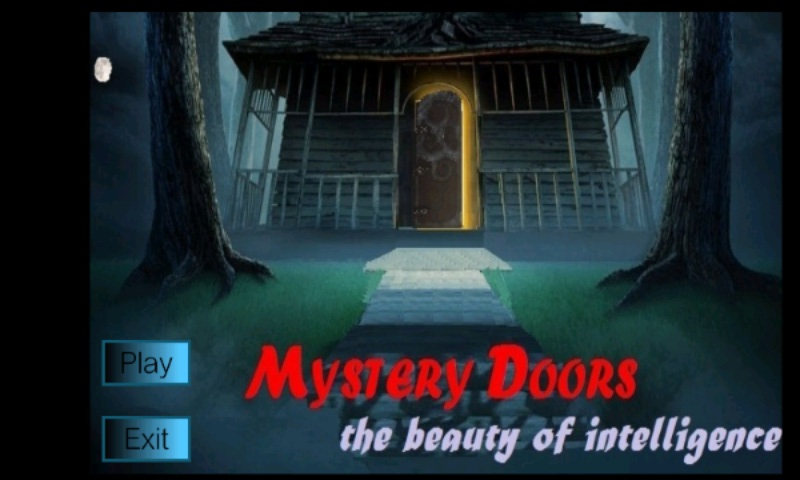
\includegraphics[width=10cm,height=6cm]{1.jpg}
	\caption{Introduction}
\end{figure}
\begin{figure}[htbp]
	\centering
	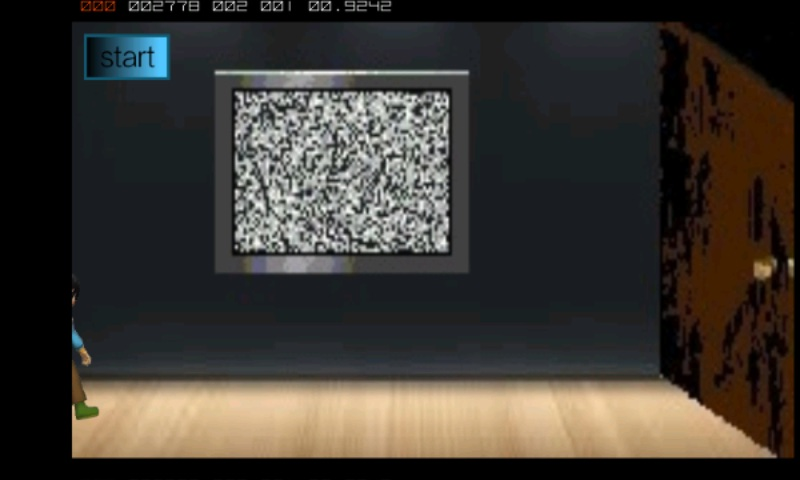
\includegraphics[width=10cm,height=6cm]{2.jpg}
	\caption{Introduction}
\end{figure}
\begin{figure}[htbp]
	\centering
	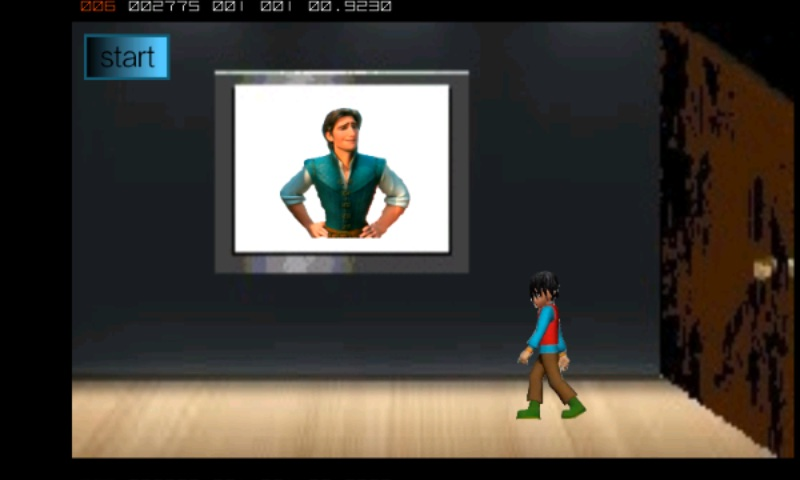
\includegraphics[width=10cm,height=6cm]{3.jpg}
	\caption{Introduction}
\end{figure}

\vspace{6cm}





\subsection{Level1}
\hspace{1cm}After the completion of the introduction the CONTINUE button is enabled.
When the user clicks on the CONTINUE button the first question of the first level
is displayed which is shown in the fig.6.4. When the user types the right answer, the next question is unlocked.After all the 3 questions of level 1 are answered, the page is displayed that the user  has completed the first level which is shown in the fig.6.5.


\begin{figure}[htbp]
	\centering
	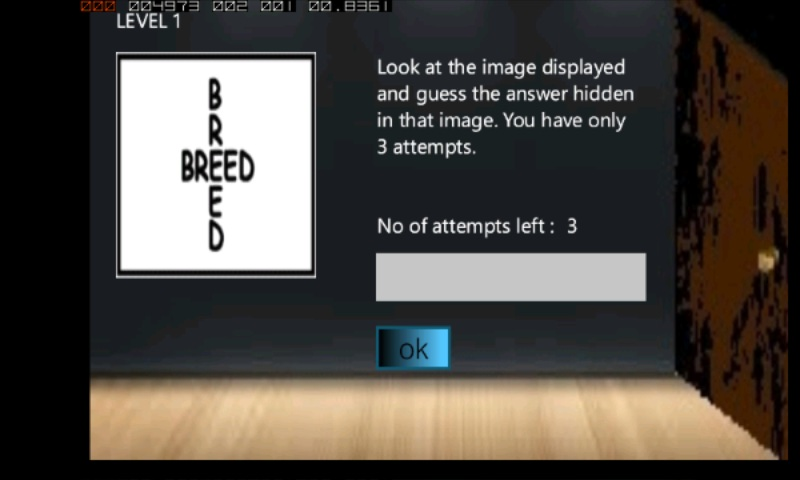
\includegraphics[width=10cm,height=6cm]{4.jpg}
	\caption{Level1}
\end{figure}

\begin{figure}[htbp]
	\centering
	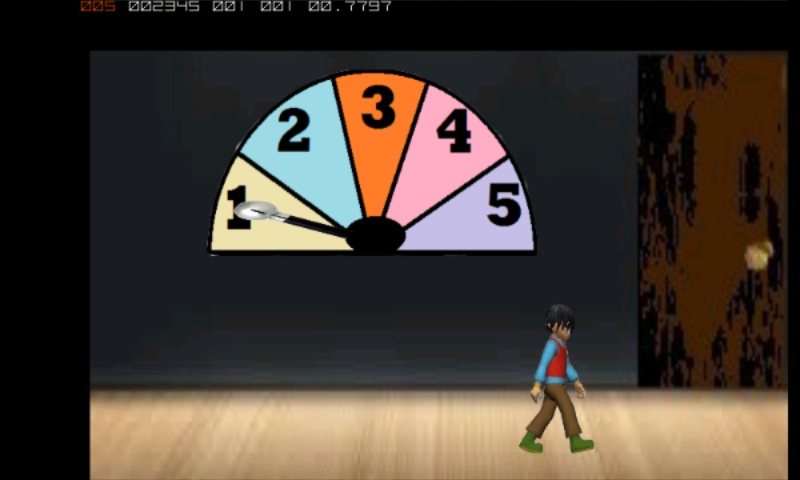
\includegraphics[width=10cm,height=6cm]{5.jpg}
	\caption{Completion of level1}
\end{figure}

\subsection{Level2}
\hspace{1cm}The fig.6.6 shows the sample of the question displayed to the user, the text field is provided 
to write the correct answer. If the answer is wrong, the user is notified.   
After all the 3 questions of level 2 are answered, the page is displayed that the user  has completed the second level which is shown in the fig.6.7.

\begin{figure}[htbp]
	\centering
	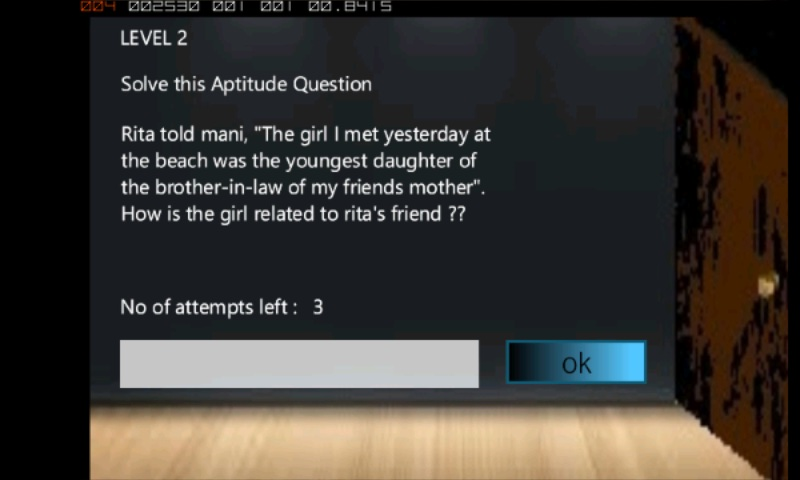
\includegraphics[width=10cm,height=6cm]{6.jpg}
	\caption{Level2}
\end{figure}
\begin{figure}[htbp]
	\centering
	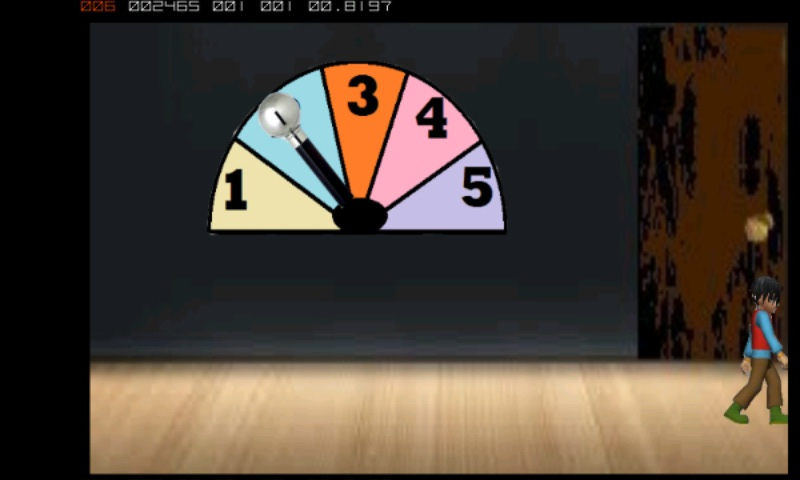
\includegraphics[width=10cm,height=6cm]{7.jpg}
	\caption{Completion of level 2}
\end{figure}

\section{Prototype : 2}
\hspace{1cm} This includes result and screenshots of third level and fourth level.
\subsection{Level3}
\hspace{1cm}The fig.6.8 shows the screenshot of the 3rd level. Here we have introduced a time-constraint and a bonus life for the user. In this level we have introduced the concept of the “password”. When the user answers 3 questions correctly, the jumbled password is unveiled, the user should then form this into the meaningful word which is shown in fig.6.9.
After all the 3 questions of level 3 are answered, the page is displayed that the user  has completed the third level which is shown in the fig.6.10.


\begin{figure}[htbp]
	\centering
	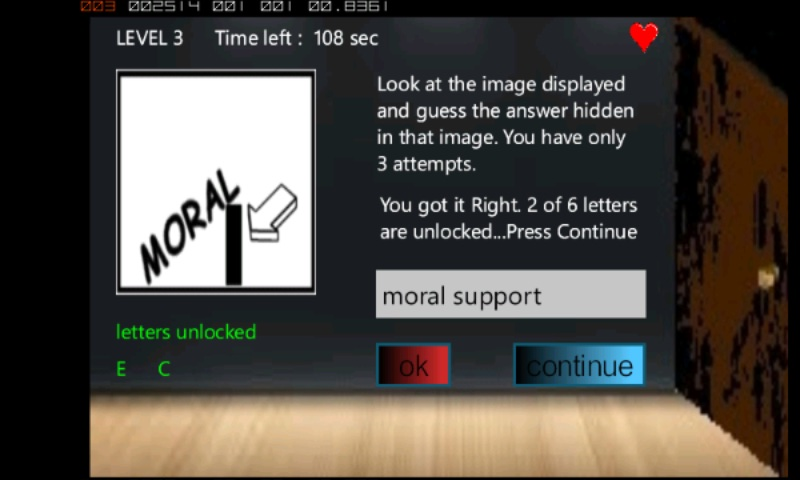
\includegraphics[width=10cm,height=6cm]{8.jpg}
	\caption{Level3}
\end{figure}
\begin{figure}[htbp]
	\centering
	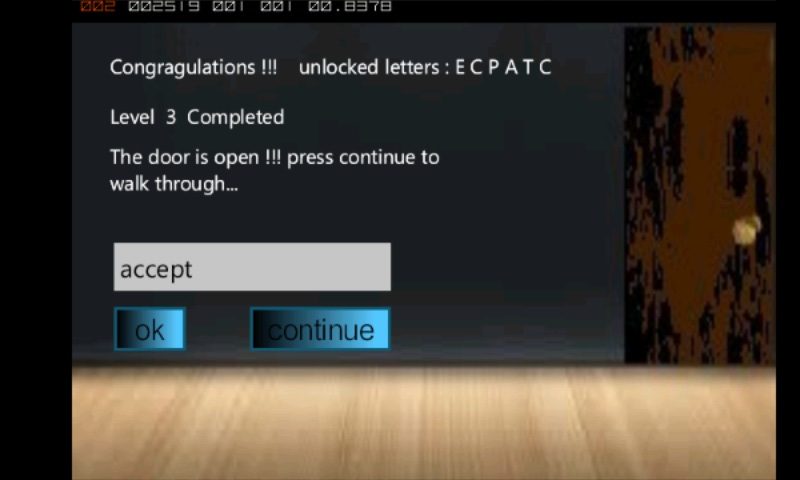
\includegraphics[width=10cm,height=6cm]{9.jpg}
	\caption{Level3}
\end{figure}
\begin{figure}[htbp]
	\centering
	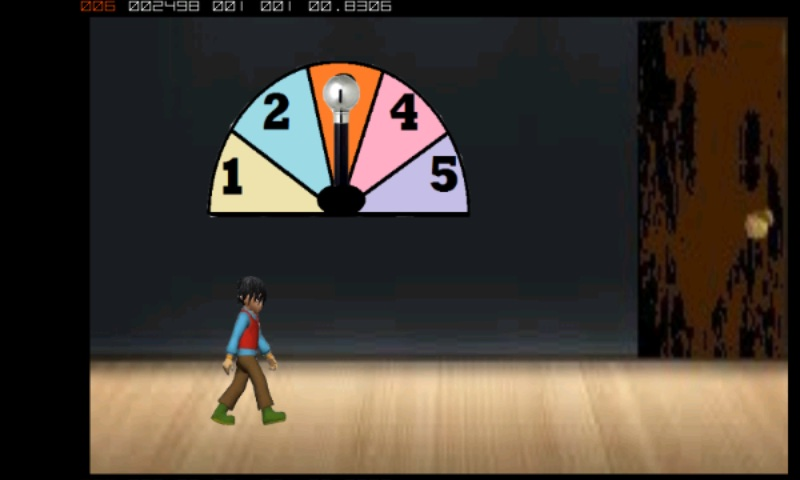
\includegraphics[width=10cm,height=6cm]{10.jpg}
	\caption{Completion of level 3}
\end{figure}

\vspace{6cm}

\subsection{Level4}
\hspace{1cm}The fig.6.11 shows the 4th level of the game. The user is given a set of images and a related image. The user is supposed to give the right answer. After all the 3 questions of level 4 are answered, the page is displayed that the user  has completed the fourth level which is shown in the fig.6.12.


\begin{figure}[htbp]
	\centering
	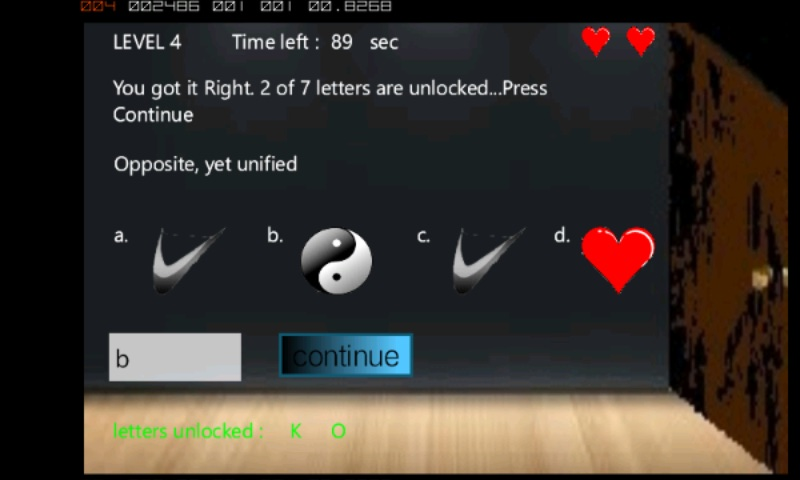
\includegraphics[width=10cm,height=6cm]{11.jpg}
	\caption{Level4}
\end{figure}
\begin{figure}[htbp]
	\centering
	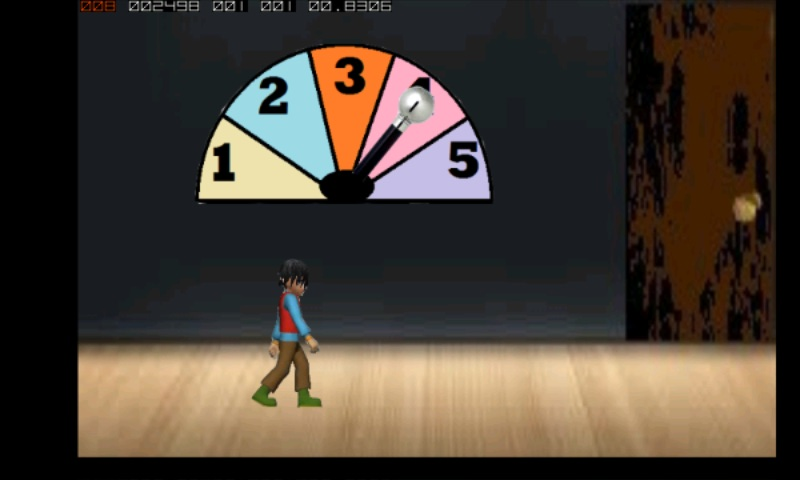
\includegraphics[width=10cm,height=6cm]{12.jpg}
	\caption{Completion of level 4}
\end{figure}


\section{Prototype : 3}
\hspace{1cm} This includes result and screenshots of fifth level and climax.

\subsection{Level5}
\hspace{1cm}The fig.6.13 shows completion of all the levels. 
\begin{figure}[htbp]
	\centering
	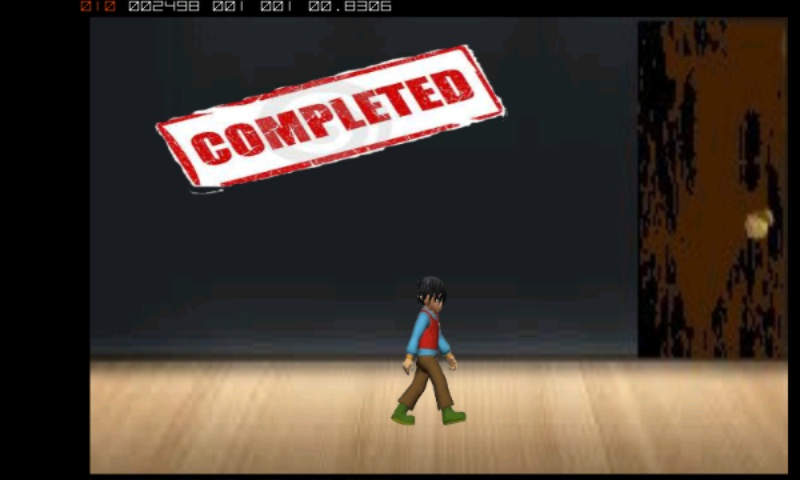
\includegraphics[width=10cm,height=6cm]{13.jpg}
	\caption{Completion of level 5}
\end{figure}
\subsection{Climax}
\hspace{1cm}The fig.6.14  shows the last scene of the game, when the user unlocks all the doors he rescues the girl.
At the end of the game, the credits are displayed which is shown in fig.6.15 and fig.6.16.
 

\begin{figure}[htbp]
	\centering
	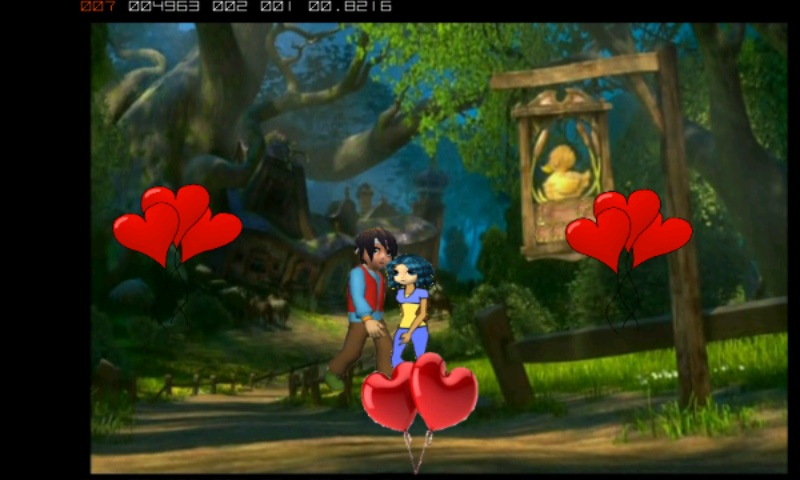
\includegraphics[width=10cm,height=6cm]{15.jpg}
	\caption{Climax}
\end{figure}
\begin{figure}[htbp]
	\centering
	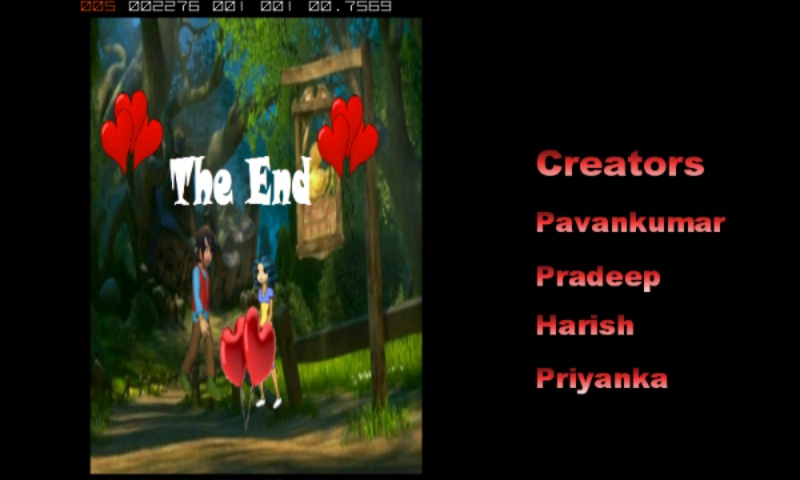
\includegraphics[width=10cm,height=6cm]{16.jpg}
	\caption{Climax}
\end{figure}
\begin{figure}[htbp]
	\centering
	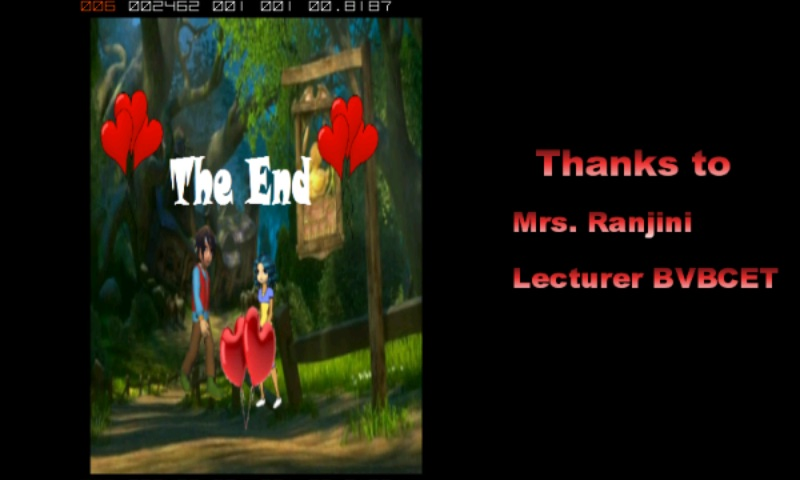
\includegraphics[width=10cm,height=6cm]{17.jpg}
	\caption{Climax}
\end{figure}
